% Seção 3: Casos de Uso

\section{Casos de Uso}
\subsection{\textit{Closed-Loop Control} no 5G}
\begin{frame}
    \frametitle{\textit{Closed-Loop Control} (CLC)}
    \begin{itemize}
        \item \textbf{Definição}: Sistema de automação que ajusta parâmetros da rede em tempo real com base em feedback contínuo.
        \item \textbf{Componentes}: Monitoramento, análise, decisão e execução.
        \item \textbf{Benefícios}: Otimização contínua da rede, melhoria na Qualidade de Serviço (QoS), resposta rápida a falhas.
    \end{itemize}
\end{frame}

\begin{frame}
    \frametitle{Aplicações de CLC no 5G}
    \begin{itemize}
        \item \textbf{\textit{Self-Organizing Networks} (SON)}: Redes que se auto-configuram, otimizam e recuperam.
        \item \textbf{Gerenciamento de Tráfego}: Ajustes automáticos para otimizar o fluxo de dados.
        \item \textbf{Manutenção Preditiva}: Prevenção de falhas com base em análise contínua de dados.
    \end{itemize}
    \begin{figure}
        \centering
        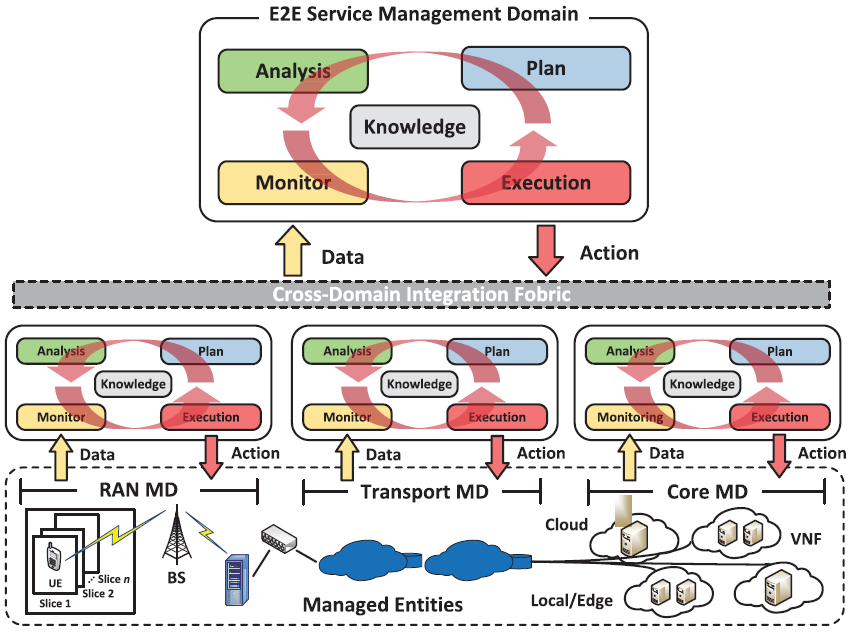
\includegraphics[width=0.45\linewidth]{figs/CLC_example.png}
        \caption{Estrutura proposta pelo ETSI ZSM\footcite{CLC_example}}
    \end{figure}
\end{frame}

\subsection{Indústria 4.0 e 5G}
\begin{frame}
    \frametitle{Indústria 4.0}
    \begin{itemize}
        \item \textbf{Definição}: Fusão de tecnologias digitais, físicas e biológicas, impulsionada pela conectividade e automação.
        \item \textbf{Componentes}: IoT, robótica avançada, \textit{big data}, IA, e computação em nuvem.
        \item \textbf{Objetivo}: Produção mais inteligente, eficiente e flexível.
    \end{itemize}
\end{frame}

\begin{frame}
    \frametitle{O Papel do 5G na Indústria 4.0}
    \begin{itemize}
        \item \textbf{Conectividade Onipresente}: Conexão confiável para um grande número de dispositivos e sensores.
        \item \textbf{Baixa Latência}: Comunicação quase em tempo real, essencial para automação.
        \item \textbf{Customização e Flexibilidade}: Produção adaptável às demandas do mercado.
    \end{itemize}
\end{frame}

\begin{frame}
    \frametitle{Casos de Uso do 5G na Indústria 4.0}
    \begin{itemize}
        \item \textbf{Automação e Robótica}: Robôs conectados em tempo real.
        \item \textbf{Manutenção Preditiva}: Monitoramento contínuo de equipamentos para prever falhas.
        \item \textbf{\textit{Supply Chain Inteligente}}: Integração e otimização em tempo real de toda a cadeia de suprimentos.
    \end{itemize}
    \begin{figure}
        \centering
        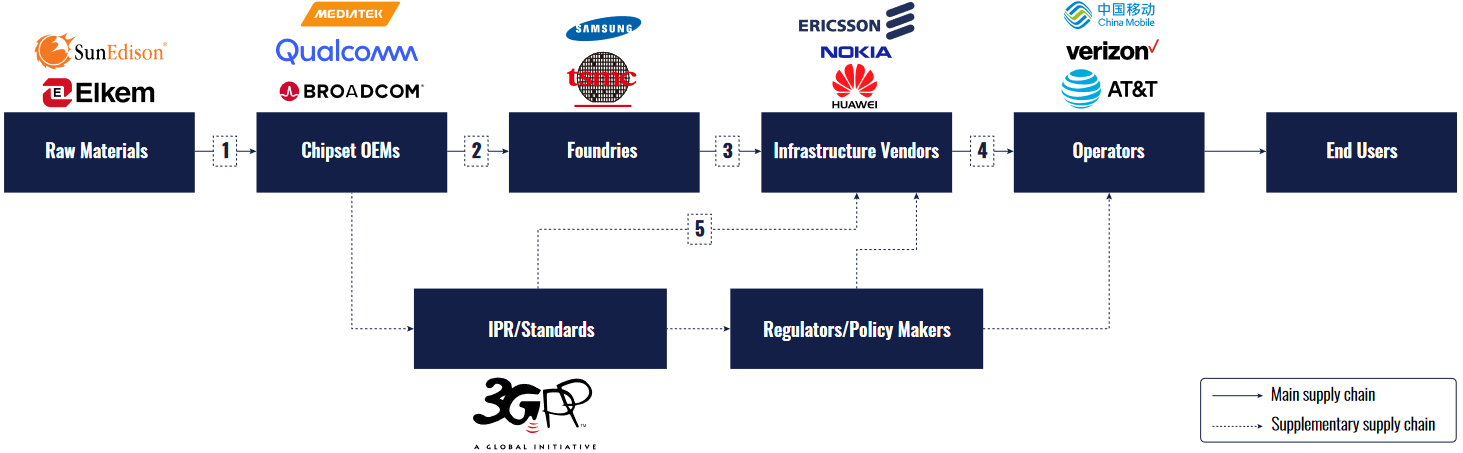
\includegraphics[width=\linewidth]{figs/supply_chain.png}
        \caption{Cadeia de suprimentos - exemplos de empresas-chave\footcite{ABI2021SupplyChain}}
    \end{figure}
\end{frame}

